\documentclass[11pt]{article}
\usepackage[margin=1in]{geometry}
\usepackage{amsmath,amssymb,amsthm,mathtools}
\usepackage{graphicx}
\usepackage{microtype}
\usepackage[hidelinks]{hyperref}
\usepackage{enumitem}
\emergencystretch=3em

\newtheorem{theorem}{Theorem}
\newtheorem{lemma}{Lemma}
\newcommand{\N}{\mathbb N}
\newcommand{\Hh}{\mathcal H}
\newcommand{\cF}{\mathcal F}
\newcommand{\cU}{\mathcal U}

\title{A Category-(c) Normalizable Frame:\\
An Explicit Counterexample to Conjecture 3.14}
\author{Automated mathematics run \texttt{fa\_banach\_001}, lane 5}
\date{August 9, 2026}

\begin{document}
\maketitle

\begin{center}
\fbox{\parbox{0.9\textwidth}{\textbf{Status.}
Candidate counterexample, likely valid, pending expert review.  An explicit
normalizable frame in $\ell^2(\N)$ belongs to category (c) of Yu's
Theorem 3.13, disproving Conjecture 3.14.}}
\end{center}

\begin{abstract}
We construct a countable frame whose normalization is again a frame and whose
successive norm bands are all frames, with summable optimal lower bounds and
optimal upper bounds converging to zero.  Every frame operator is diagonal in
the standard basis and all optimal bounds are computed exactly.  The
construction gives a full negative answer to Conjecture 3.14 in
Yu's \emph{Frame-normalizable Sequences}.
\end{abstract}

\section{Source problem}

Let $(x_n)$ be a sequence of nonzero vectors in a Hilbert space.  It is
\emph{frame-normalizable} if the unit-vector sequence
$(x_n/\|x_n\|)$ is a frame, and it is a \emph{normalizable frame} if both
$(x_n)$ and its normalization are frames.

Yu's Theorem 3.13 divides normalizable frames into three categories.  Its
category (c) consists of those for which there are positive numbers
$\delta_k\downarrow0$ such that every norm band
\[
 \cF_k=\{x_n:\delta_{k+1}\le \|x_n\|<\delta_k\}
\]
is a frame.  If $A_k,B_k$ are the optimal lower and upper frame bounds of
$\cF_k$, the theorem also proves $(A_k)\in\ell^1$ and $B_k\to0$.

\begin{figure}[ht]
  \centering
  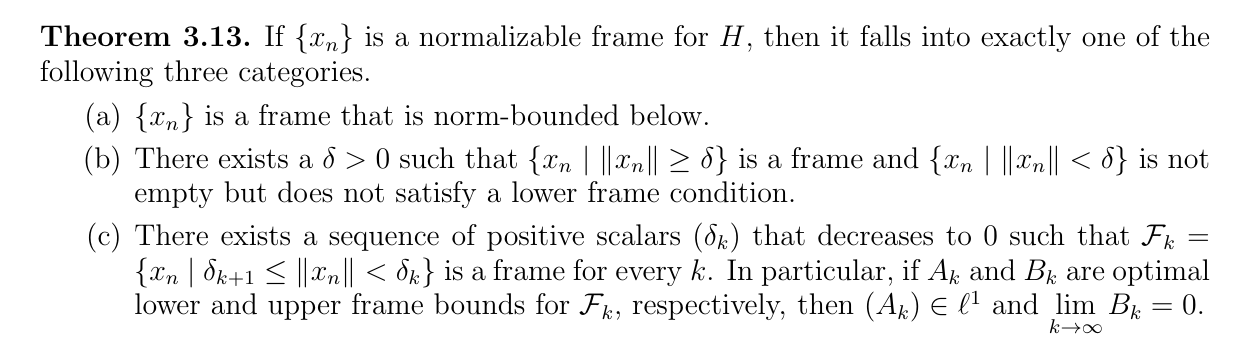
\includegraphics[width=0.96\textwidth]{figures/category_c_theorem_crop.png}
  \caption{The definition and necessary bounds for category (c) in
  Yu's Theorem 3.13~\cite[p.~8]{Yu}.}
  \label{fig:category-c}
\end{figure}

Immediately after its proof, Yu proposes the following conjecture:
\begin{quote}
``There does not exist a normalizable frame belonging to category (c) in
Theorem 3.13.''
\end{quote}

\begin{figure}[ht]
  \centering
  
\includegraphics[width=0.96\textwidth]{figures/open_problem_crop.png}
  \caption{Conjecture 3.14 in the source paper~\cite[p.~9]{Yu}.}
  \label{fig:conjecture}
\end{figure}

\section{Proof intuition}

A single norm band must be a frame for the whole Hilbert space even though
all its vectors have one small common norm.  The normalized version of that
band can therefore have a very poor lower frame bound.  We realize this with
two vectors on each of infinitely many orthogonal coordinate pairs.  Their
opposite signs cancel all off-diagonal terms, leaving a block frame operator
that has weight nearly $2$ on a chosen infinite set and a small weight $a_k$
on its complement.

The chosen infinite sets partition the coordinates.  Thus, when all
normalized bands are united, every coordinate receives one large weight and
the sum of all remaining small weights.  After scaling the $k$th band by
$r_k$, the common small weights still sum to a strictly positive number.
This simultaneously makes the original sequence and its normalization
frames, while geometrically separated norms make the bands exact.

\section{Counterexample theorem}

For a subset $E\subseteq\N$, write $P_E$ for the orthogonal projection onto
$\overline{\operatorname{span}}\{e_j:j\in E\}$.

\begin{theorem}\label{thm:main}
There exists a normalizable frame in $\ell^2(\N)$ belonging to category (c)
of Theorem 3.13.  More precisely, it can be chosen so that its normalized
sequence has optimal frame bounds $2$ and $3$, the original sequence has
optimal frame bounds $1/7$ and $11/28$, and its norm bands have optimal bounds
\[
 A_k=2^{-3k},\qquad
 B_k=4^{-k}(2-2^{-k}).
\]
Consequently Conjecture 3.14 is false.
\end{theorem}

\begin{proof}
Let $\Hh=\ell^2(\N)$ with its standard orthonormal basis $(e_j)_{j\ge1}$.
For instance, take the explicit partition
\[
 E_k=\{2^{k-1}(2m-1):m\ge1\},\qquad
 \N=\bigsqcup_{k\ge1}E_k.
\]
Every $E_k$ is infinite.  Both $E_k$ and $E_k^c$ are countably
infinite, so let $\sigma_k:E_k\to E_k^c$ match their increasing
enumerations.  Put
\[
 a_k=2^{-k},\qquad r_k=2^{-k}.
\]
For $p\in E_k$, define two unit vectors
\begin{equation}\label{eq:u-def}
 u_{k,p}^{\pm}
 =\sqrt{1-\frac{a_k}{2}}\,e_p
 \mathbin{\pm}\sqrt{\frac{a_k}{2}}\,e_{\sigma_k(p)},
\end{equation}
and let $\cU_k=(u_{k,p}^{\pm})_{p\in E_k}$.  Finally set
\begin{equation}\label{eq:x-def}
 x_{k,p}^{\pm}=r_k u_{k,p}^{\pm}.
\end{equation}
This countable double family may of course be enumerated as a sequence.

We first compute the frame operator of one unit-vector block.  For fixed
$k,p$, the opposite signs in \eqref{eq:u-def} cancel the cross terms:
\begin{equation}\label{eq:pair-operator}
 u_{k,p}^{+}\otimes u_{k,p}^{+}
 +u_{k,p}^{-}\otimes u_{k,p}^{-}
 =(2-a_k)e_p\otimes e_p
 +a_k e_{\sigma_k(p)}\otimes e_{\sigma_k(p)}.
\end{equation}
For distinct $p\in E_k$, the pairs
$\{p,\sigma_k(p)\}$ are disjoint.  Since $\sigma_k$ maps $E_k$ onto its
complement, summing \eqref{eq:pair-operator} gives the exact block operator
\begin{equation}\label{eq:Sk}
 S_k=a_kI+(2-2a_k)P_{E_k}.
\end{equation}
Thus $\cU_k$ is a frame for $\Hh$ with optimal lower and upper bounds
$a_k$ and $2-a_k$.

The normalization of the sequence in \eqref{eq:x-def} is precisely
$\cU=\bigcup_{k\ge1}\cU_k$.  Let $j\in E_m$.  Formula \eqref{eq:Sk} and
$\sum_{k\ge1}a_k=1$ yield
\begin{equation}\label{eq:normalized-eigenvalue}
 \left(\sum_{k\ge1}S_k\right)e_j
 =\left(2-a_m+\sum_{k\ne m}a_k\right)e_j
 =(3-2a_m)e_j.
\end{equation}
These diagonal values begin at $2$ and increase to $3$.  Hence $\cU$ is a
frame with optimal bounds $2$ and $3$.

Next consider the original scaled sequence
$X=(x_{k,p}^{\pm})_{k,p,\pm}$.  Its frame operator is
\[
 T=\sum_{k\ge1}r_k^2S_k.
\]
The common diagonal contribution is
\begin{equation}\label{eq:C}
 C:=\sum_{k\ge1}r_k^2a_k
 =\sum_{k\ge1}2^{-3k}=\frac17.
\end{equation}
For $j\in E_m$, equations \eqref{eq:Sk} and \eqref{eq:C} give
\begin{equation}\label{eq:scaled-eigenvalue}
 Te_j=\left(C+r_m^2(2-2a_m)\right)e_j.
\end{equation}
The second term is nonnegative and tends to zero.  It is maximal at $m=1$,
where it equals $1/4$.  The diagonal values in
\eqref{eq:scaled-eigenvalue} therefore have infimum $1/7$ and maximum
$1/7+1/4=11/28$.  Thus $X$ is a frame with precisely those optimal bounds.
Together with \eqref{eq:normalized-eigenvalue}, this proves that $X$ is a
normalizable frame.

It remains to identify its norm bands.  All vectors in the $k$th block have
norm $r_k$.  Define
\begin{equation}\label{eq:delta}
 \delta_k=3\,2^{-(k+1)}=\frac32r_k.
\end{equation}
Then $\delta_k\downarrow0$ and
\[
 \delta_{k+1}=\frac34r_k<r_k<\frac32r_k=\delta_k.
\]
The neighboring norms satisfy $r_{k-1}=2r_k>\delta_k$ (when $k>1$) and
$r_{k+1}=r_k/2<\delta_{k+1}$; all more distant norms are farther away.
Consequently
\begin{equation}\label{eq:band}
 \{x\in X:\delta_{k+1}\le\|x\|<\delta_k\}=r_k\cU_k.
\end{equation}
By \eqref{eq:Sk}, this band is a frame with optimal bounds
\[
 A_k=r_k^2a_k=2^{-3k},\qquad
 B_k=r_k^2(2-a_k)=4^{-k}(2-2^{-k}).
\]
In particular, $\sum_kA_k=1/7$ and $B_k\to0$.  Every condition in category
(c) is satisfied, completing the counterexample.
\end{proof}

\section{Verification and scope}

The proof is exact and uses no numerical lemma.  All relevant operators are
positive and diagonal in the standard basis.  The series may therefore be
checked coordinatewise, while the uniform bounds in
\eqref{eq:normalized-eigenvalue} and \eqref{eq:scaled-eigenvalue} ensure that
the resulting quadratic forms define bounded frame operators.

The counterexample gives a full negative answer to Conjecture 3.14.  It does
not classify normalizable frames, nor does it address other open questions in
the source paper.

\section{Novelty check and review recommendation}

The local run indexes were searched for arXiv:2308.13071, the exact title,
and the category-(c) conjecture, with no duplicate result found.  Bounded web
searches on August 9, 2026 used the exact conjecture sentence, the exact title
together with ``category (c),'' and the title/author together with
``conjecture.''  They found the arXiv paper, its 2024 journal publication, an
author thesis, and unrelated later citations, but no resolution of
Conjecture 3.14 or this diagonal-block construction.  The result's novelty is
therefore plausible but remains subject to expert literature review.

Human review is strongly recommended.  The decisive checks are
\eqref{eq:pair-operator}, the three diagonal calculations
\eqref{eq:normalized-eigenvalue}--\eqref{eq:scaled-eigenvalue}, and the exact
band isolation in \eqref{eq:band}.

\begin{thebibliography}{9}
\raggedright
\bibitem{Yu}
P.-T. Yu,
\emph{Frame-normalizable sequences},
Adv. Comput. Math. \textbf{50} (2024), Paper 89;
arXiv:2308.13071;
\href{https://doi.org/10.1007/s10444-024-10182-z}{doi:10.1007/s10444-024-10182-z}.
\end{thebibliography}

\end{document}
